\documentclass{article}

% Language setting
% Replace `english' with e.g. `spanish' to change the document language
\usepackage[english]{babel}
\usepackage{amsfonts}

% Set page size and margins
% Replace `letterpaper' with `a4paper' for UK/EU standard size
\usepackage[a4paper,top=2cm,bottom=2cm,left=3cm,right=3cm,marginparwidth=1.75cm]{geometry}

% Useful packages
\usepackage{amsmath}
\usepackage{graphicx}
\usepackage[colorlinks=true, allcolors=blue]{hyperref}

\title{RA-MIRI Assignment 1: Galton box}
\author{Lapeyra Amat, Joan}

\begin{document}
\maketitle

Source code: \url{https://github.com/jlapeyra/RA-assignments/tree/main/assignment-1/src}

\section{Implementation}
I implemented the Galton box in Python. The program goes as follows. Given $n, m \in \mathbb{Z}^+$, drop a ball into the box $m$ times. Each drop consists of moving the ball $n$ times. Each move is a random choice between left and right with equal probability, namely $1/2$. I used the same notation as in the statement, where the position of a ball is encoded in a pair $(i,j)$, the ball starts at $(0,0)$, a move to the left is $(i+1,j)$ and a move to the right is $(i,j+1)$. For each ball, I store the final position $i$ ($j$ is redundant because $i+j=n$). Then I plot using \texttt{matplotlib} the empirical probability of each $i$, i.e. the rate of balls that fell on position $(i,n-i)$. Over this bar plot, I print the normal distribution $\mathcal{N}(\mu=\frac{n}{2}, \sigma^2=\frac{n}{4})$ using \texttt{scipy}.

\section{Results}

The central limit theorem explains that the sum of a large number of independent random variables (like each step) will tend to form a normal distribution, regardless of the underlying distribution of the individual events (in this case, left or right).

In a Galton box, as each ball goes through numerous steps and encounters many random binary choices, the sum of these independent decisions creates the bell-shaped curve of a normal distribution.

In figure \ref{fig:6-steps} we see different plots of a Galton box with 6 steps. As expected, the larger the sample (number of balls thrown), the closer the random binomial distribution is to a normal probability density function. In addition, the smaller the sample, the more random is the distribution, i.e. the more different are different runs of the same experiment.

In figures \ref{fig:12-steps}, \ref{fig:20-steps} and \ref{fig:40-steps}, we see the same plots for Galton boxes of 12, 20 and 40 steps. The behaviour is very similar: the random distribution tends to a normal probability density function with the sample size.


\begin{figure}
    \centering
    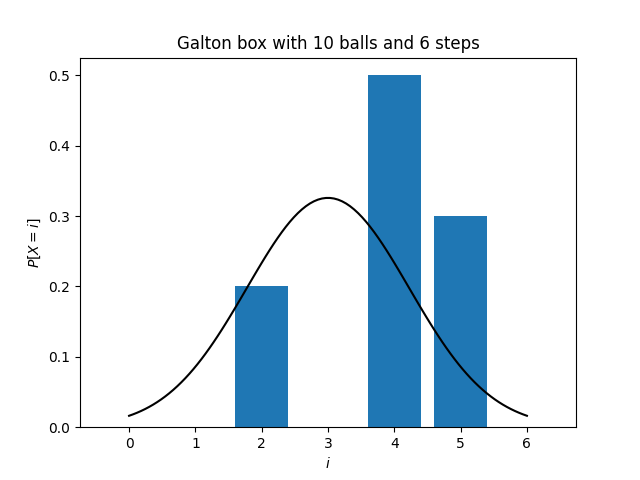
\includegraphics[width=0.32\linewidth]{plots/6-10-a.png}
    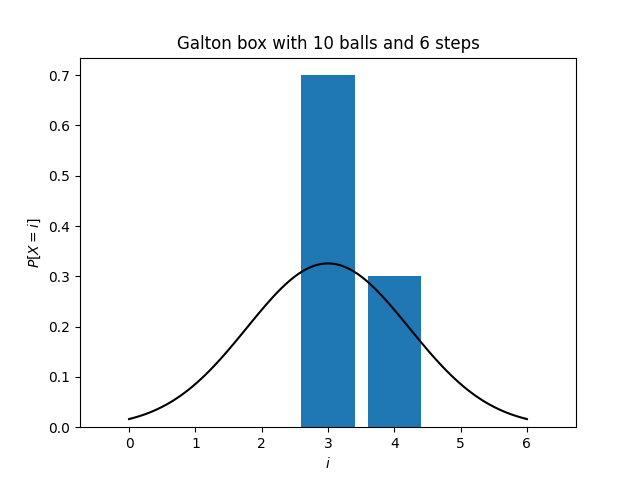
\includegraphics[width=0.32\linewidth]{plots/6-10-b.png}
    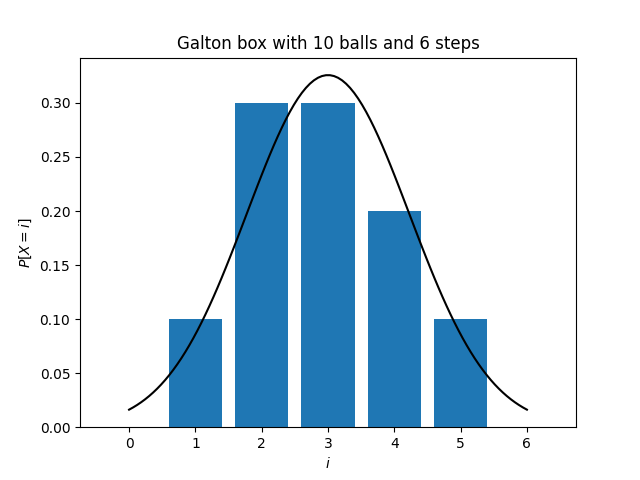
\includegraphics[width=0.32\linewidth]{plots/6-10-c.png}
    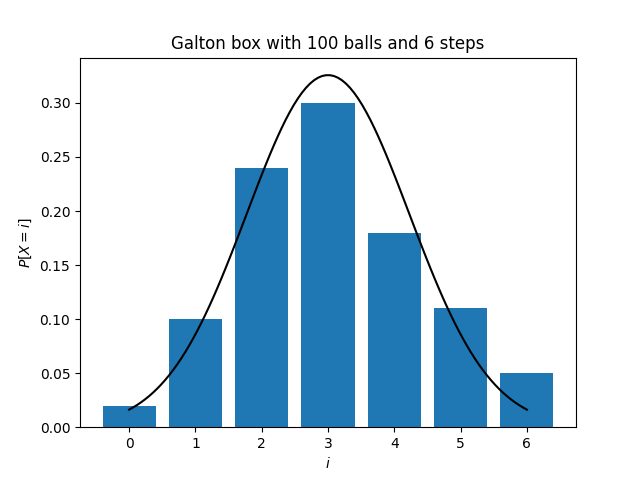
\includegraphics[width=0.32\linewidth]{plots/6-100-a.png}
    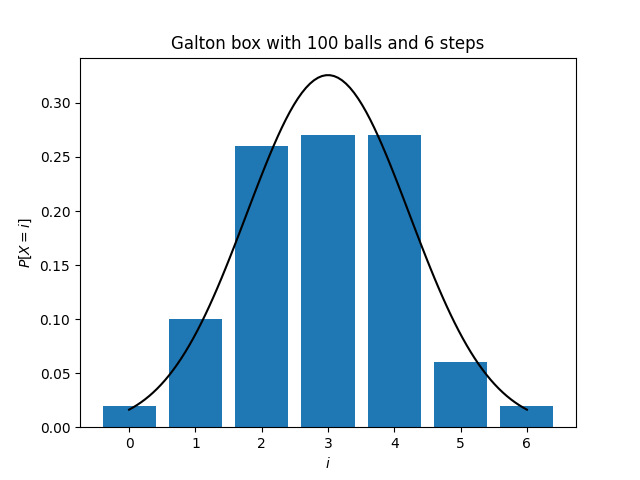
\includegraphics[width=0.32\linewidth]{plots/6-100-b.png}
    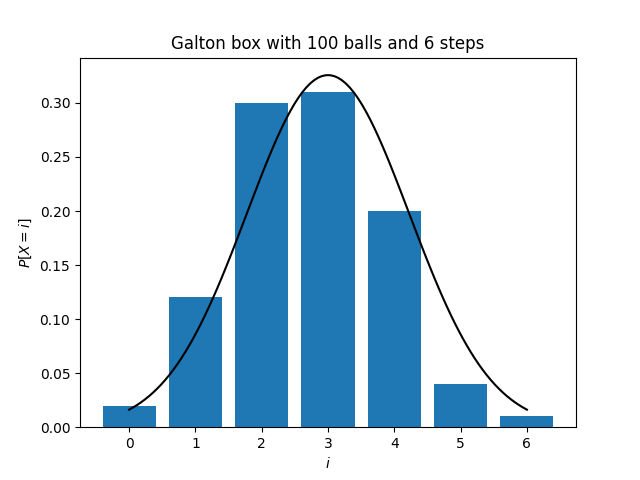
\includegraphics[width=0.32\linewidth]{plots/6-100-c.png}
    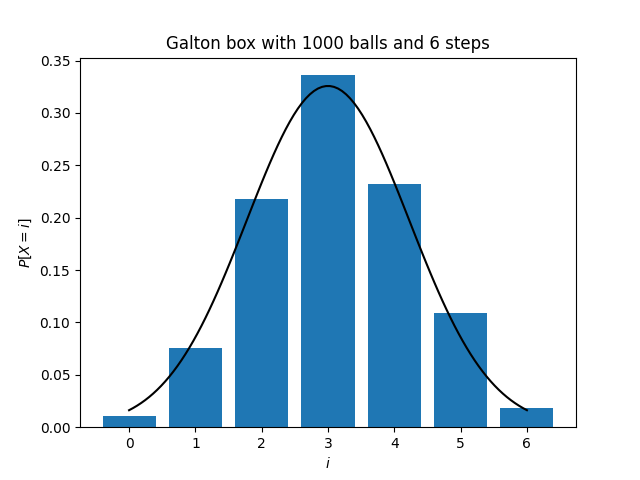
\includegraphics[width=0.32\linewidth]{plots/6-1000-a.png}
    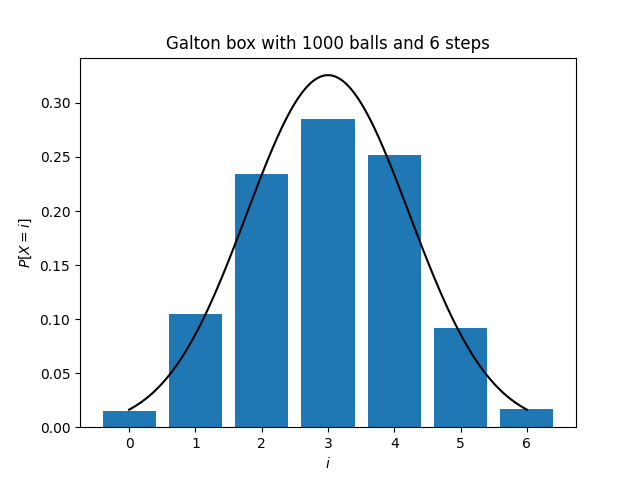
\includegraphics[width=0.32\linewidth]{plots/6-1000-b.png}
    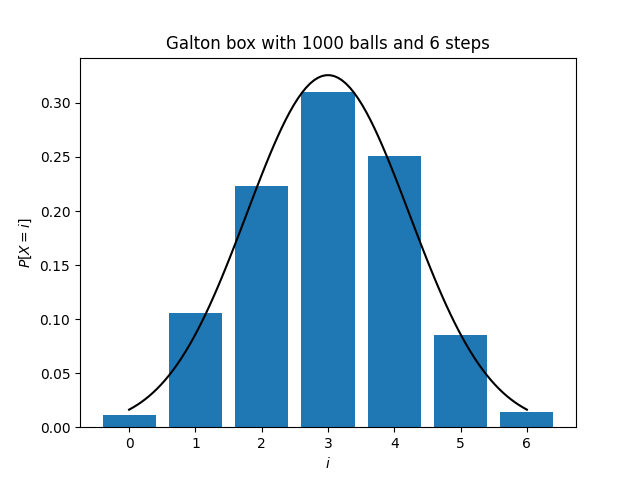
\includegraphics[width=0.32\linewidth]{plots/6-1000-c.png}
    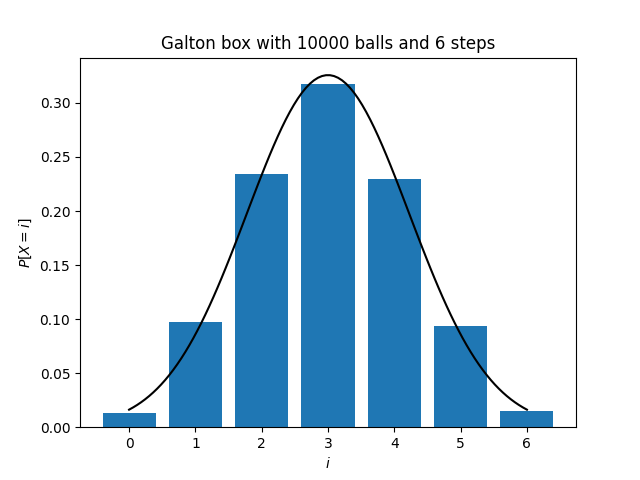
\includegraphics[width=0.32\linewidth]{plots/6-10000-a.png}
    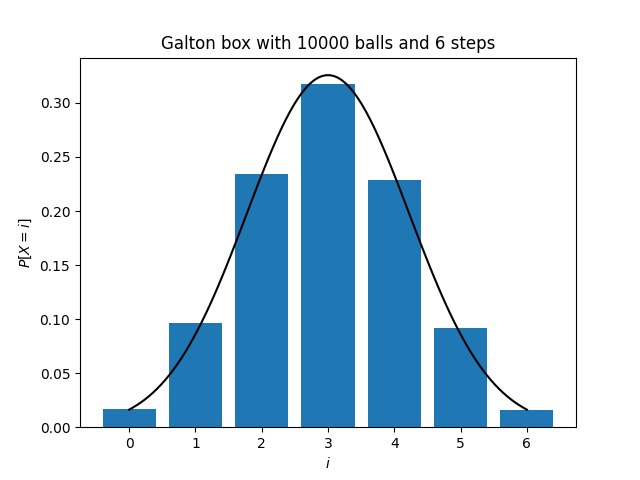
\includegraphics[width=0.32\linewidth]{plots/6-10000-b.png}
    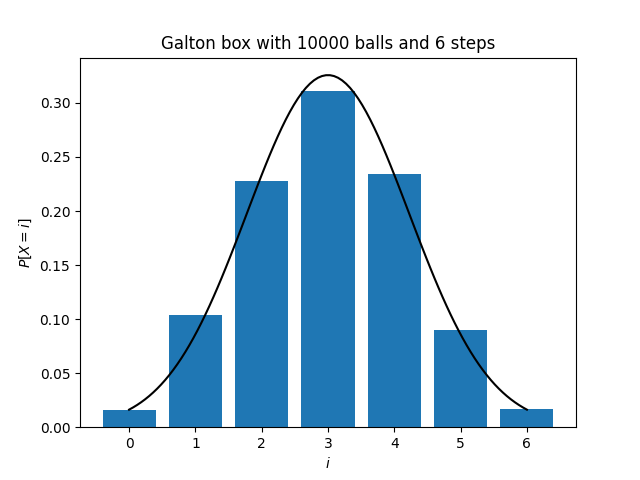
\includegraphics[width=0.32\linewidth]{plots/6-10000-c.png}
    \caption{Probability distribution of a Galton box with 6 steps. Each row has 3 runs of a given number of samples (balls thrown): 10, 100, 1,000 and 10,000.}
    \label{fig:6-steps}
\end{figure}

\begin{figure}
    \centering
    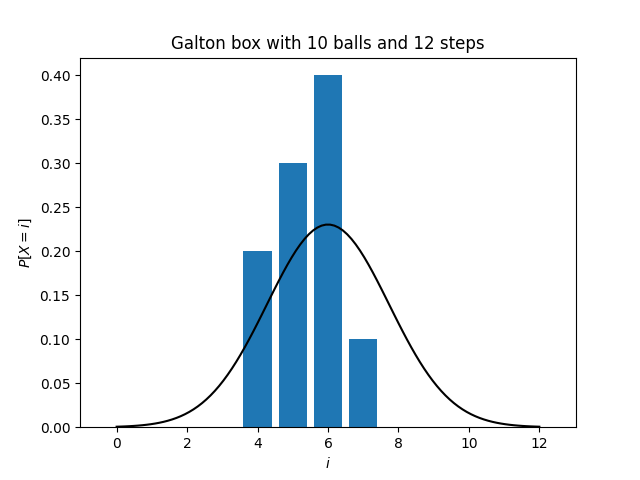
\includegraphics[width=0.48\linewidth]{plots/12-10-a.png}
    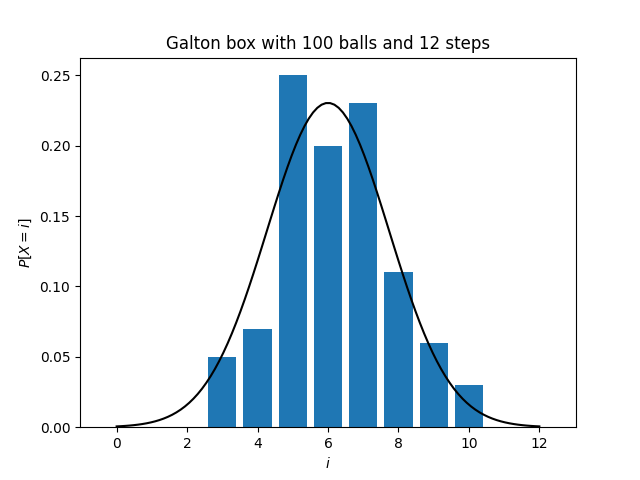
\includegraphics[width=0.48\linewidth]{plots/12-100-a.png}
    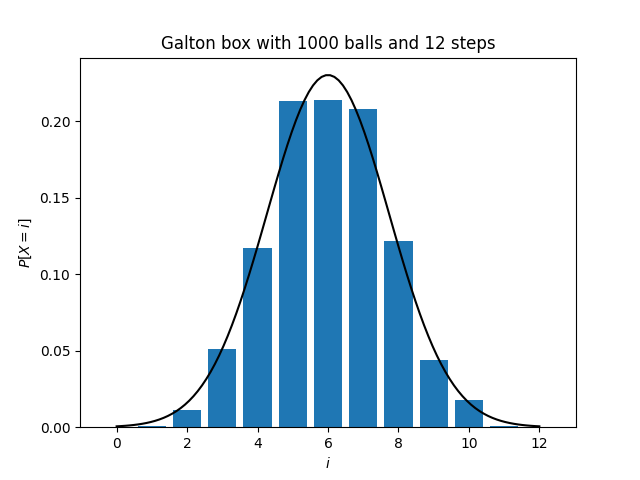
\includegraphics[width=0.48\linewidth]{plots/12-1000-a.png}
    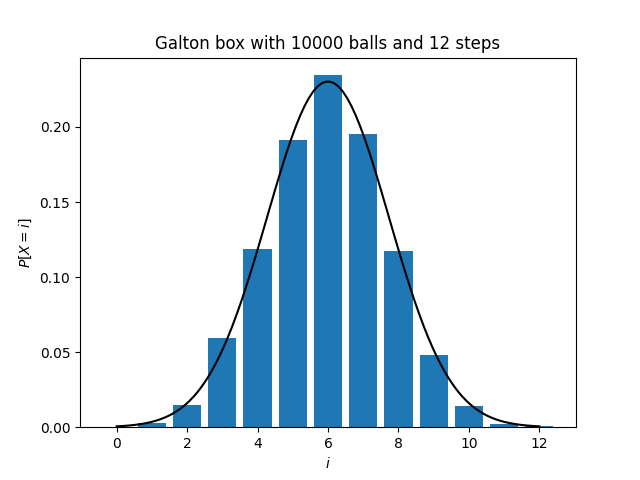
\includegraphics[width=0.48\linewidth]{plots/12-10000-a.png}
    \caption{Probability distribution of a Galton box with 12 steps. Each plot has a different number of samples (balls thrown): 10, 100, 1,000 and 10,000.}
    \label{fig:12-steps}
\end{figure}

\begin{figure}
    \centering
    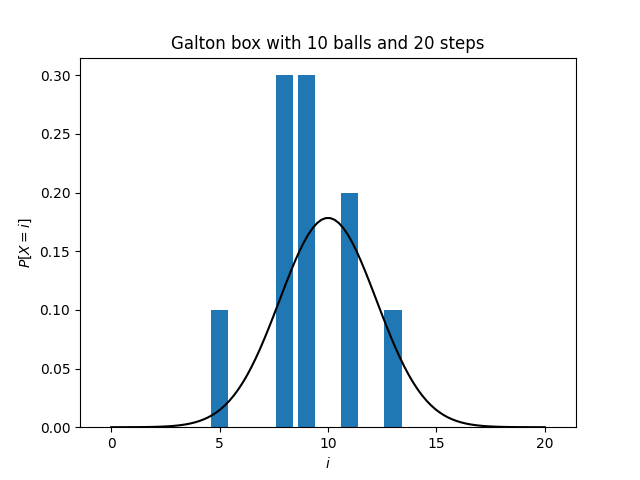
\includegraphics[width=0.48\linewidth]{plots/20-10-a.png}
    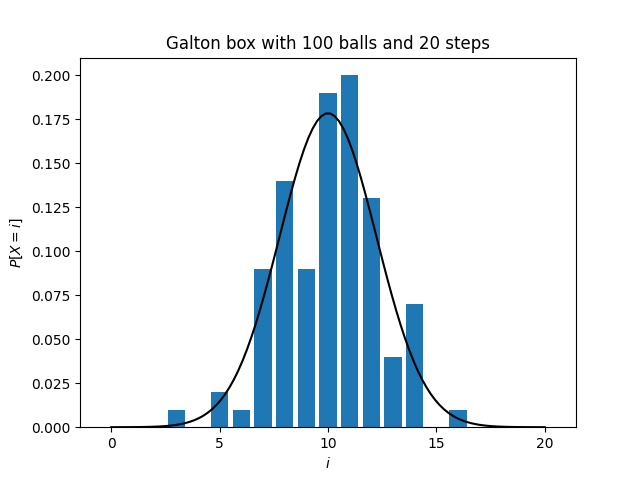
\includegraphics[width=0.48\linewidth]{plots/20-100-a.png}
    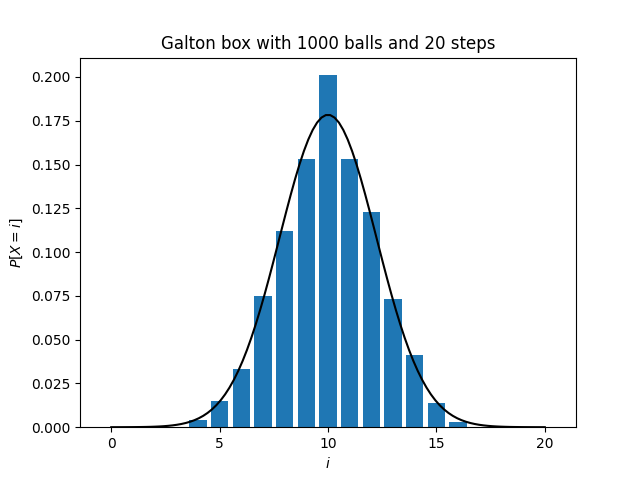
\includegraphics[width=0.48\linewidth]{plots/20-1000-a.png}
    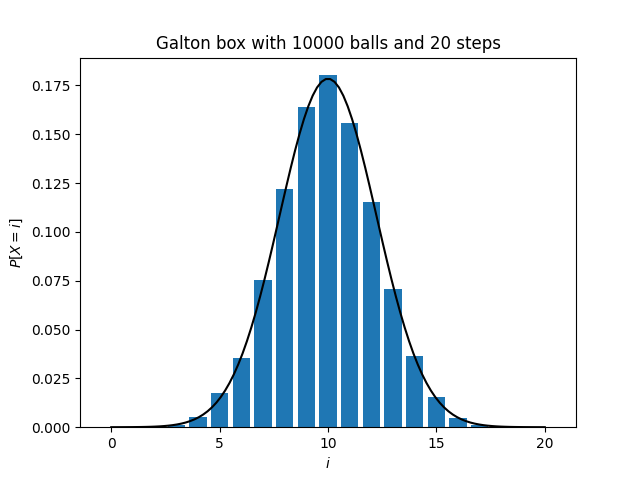
\includegraphics[width=0.48\linewidth]{plots/20-10000-a.png}
    \caption{Probability distribution of a Galton box with 20 steps. Each plot has a different number of samples (balls thrown): 10, 100, 1,000 and 10,000.}
    \label{fig:20-steps}
\end{figure}

\begin{figure}
    \centering
    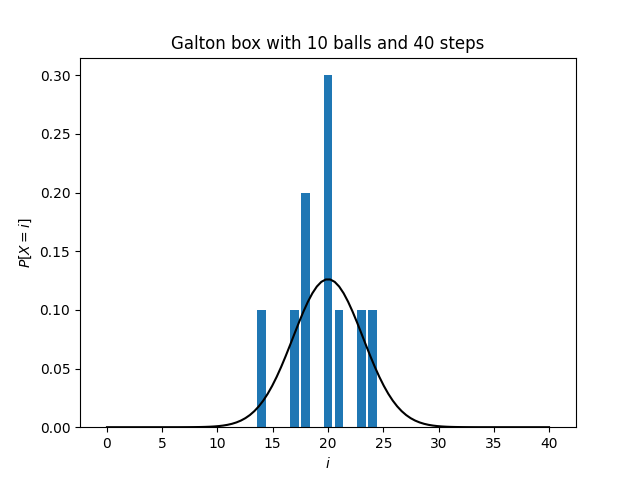
\includegraphics[width=0.48\linewidth]{plots/40-10-a.png}
    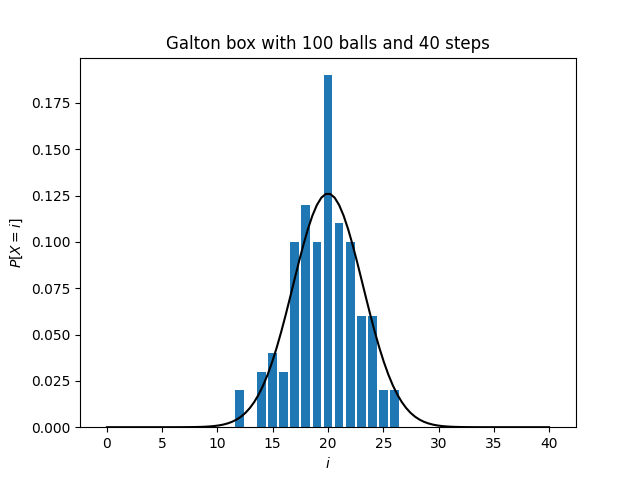
\includegraphics[width=0.48\linewidth]{plots/40-100-a.png}
    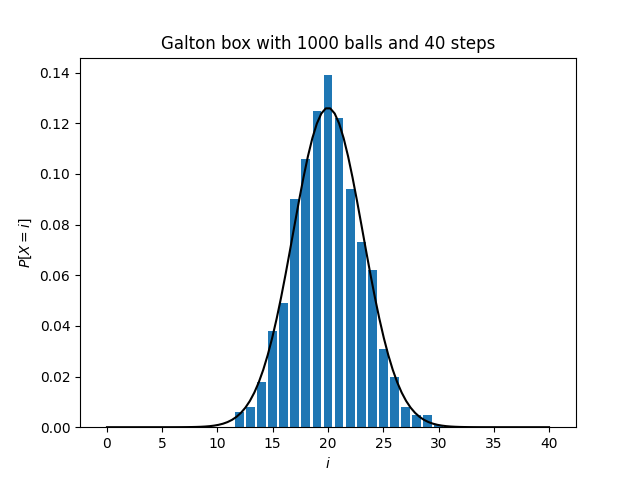
\includegraphics[width=0.48\linewidth]{plots/40-1000-a.png}
    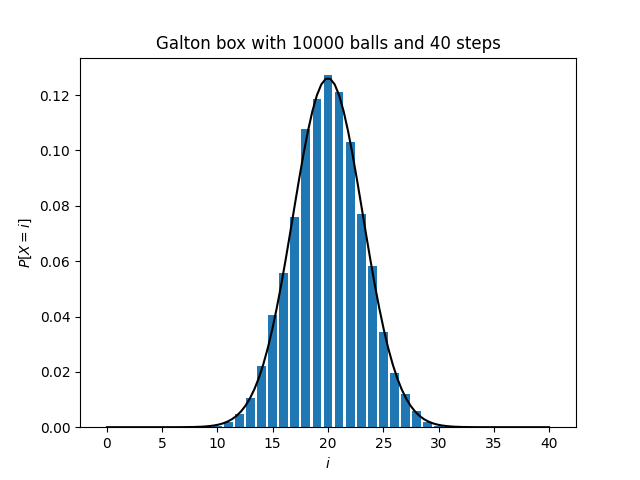
\includegraphics[width=0.48\linewidth]{plots/40-10000-a.png}
    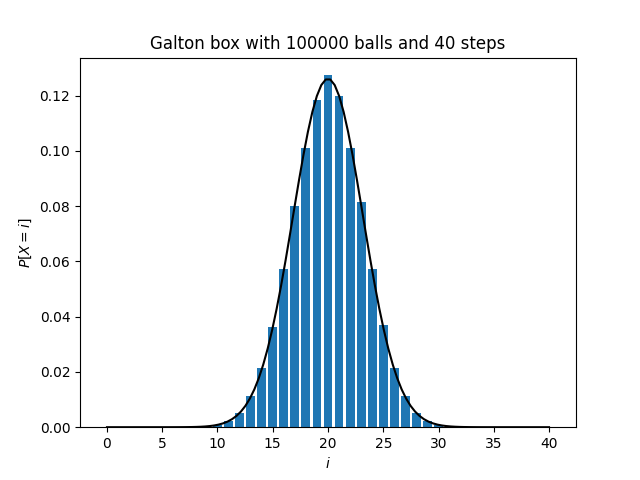
\includegraphics[width=0.48\linewidth]{plots/40-100000-a.png}
    \caption{Probability distribution of a Galton box with 40 steps. Each plot has a different number of samples (balls thrown): 10, 100, 1,000, 10,000 and 100,000.}
    \label{fig:40-steps}
\end{figure}

\end{document}